\section{Baseline and Methods}

\subsection{Model Overview}

Three models are implemented and evaluated. Table~\ref{tab:model_summary} provides a high-level comparison.

\begin{table}[H]
    \centering
    \caption{Summary of the three models compared in this assignment.}
    \label{tab:model_summary}
    \begin{tabularx}{\textwidth}{l l r r l}
        \toprule
        \textbf{Experiment} & \textbf{Architecture} & \textbf{Total Params} & \textbf{Trainable} & \textbf{Pretrained} \\
        \midrule
        EXP-1 & BiLSTM (scratch)          & 4,567,557  & 4,567,557 (100\%)   & No \\
        EXP-2 & DistilBERT (frozen head)  & 66,957,317 & 594,437 (0.89\%)    & Yes \\
        EXP-3 & DistilBERT (full fine-tune)& 66,957,317 & 66,957,317 (100\%) & Yes \\
        \bottomrule
    \end{tabularx}
\end{table}

\subsection{EXP-1: BiLSTM Baseline (from Scratch)}

The BiLSTM model is a compact recurrent sequence classifier trained entirely from scratch. Its architecture is as follows:

\begin{enumerate}
    \item \textbf{Embedding layer:} \texttt{nn.Embedding(30522, 128, padding\_idx=0)} — maps each token index to a 128-dimensional dense vector. The embedding weights are randomly initialised and learned during training.
    \item \textbf{Bidirectional LSTM:} 2-layer \texttt{nn.LSTM(128, 128, num\_layers=2, bidirectional=True, dropout=0.3)} — processes the token sequence in both directions. At each layer, the hidden dimension is 128 per direction, yielding a concatenated output dimension of 256.
    \item \textbf{Sequence aggregation:} The hidden states from the final forward and backward LSTM cells (not the output sequence) are concatenated to form a fixed 256-dimensional sentence vector.
    \item \textbf{Classification head:} \texttt{Dropout(0.3)} $\to$ \texttt{Linear(256, 5)}.
\end{enumerate}

The forward pass uses \texttt{pack\_padded\_sequence} to skip padding tokens during recurrent computation. The sequence lengths are derived from the \texttt{attention\_mask} provided by the tokenizer.

\begin{figure}[H]
    \centering
    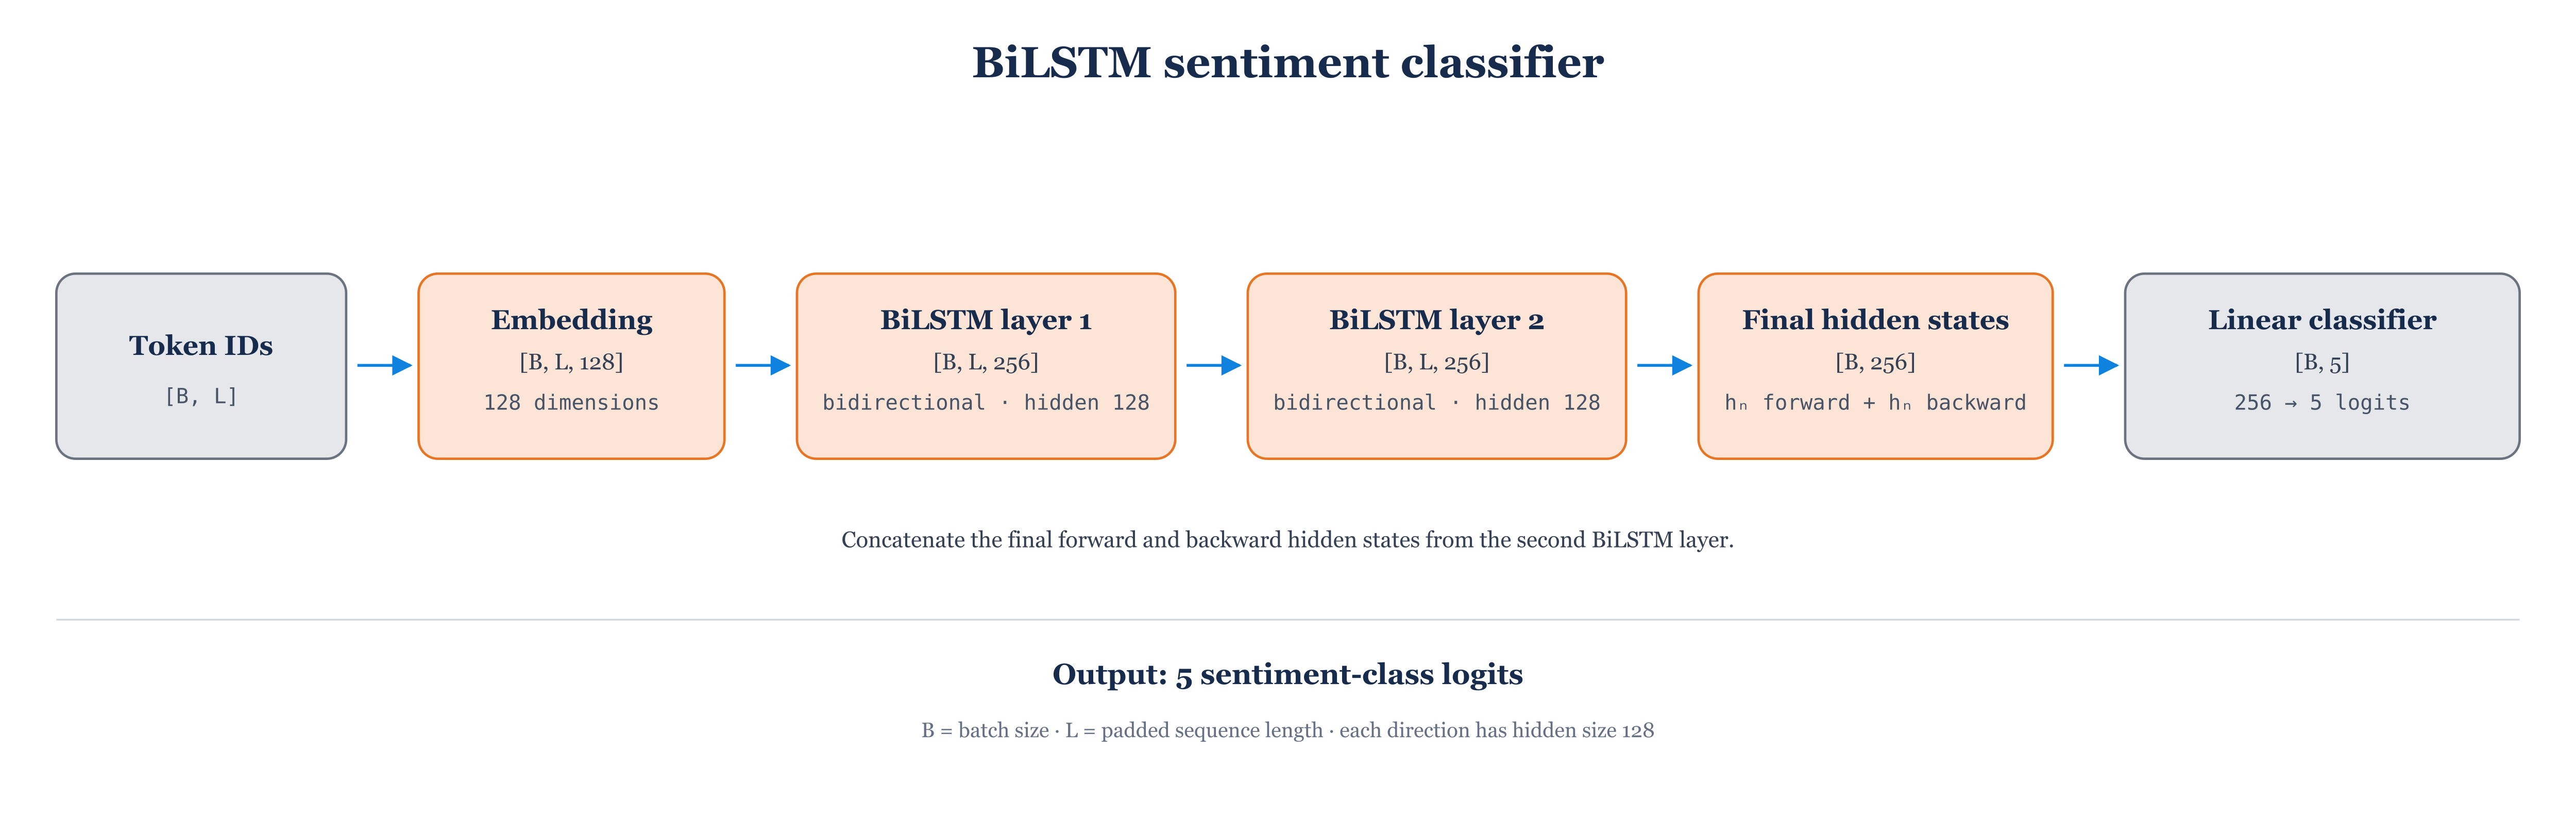
\includegraphics[width=0.60\textwidth]{../../Assignment2/diagram-models/bilstm-model.png}
    \caption{Architecture diagram of the BiLSTM classifier (EXP-1).}
    \label{fig:bilstm_arch}
\end{figure}

\subsection{EXP-2 and EXP-3: DistilBERT Classifier}

Both EXP-2 and EXP-3 use the \textbf{same model class} (\texttt{DistilBertClassifier}) with identical architecture. The only difference is which parameters are frozen during training.

\subsubsection{Backbone}

The backbone is \texttt{distilbert-base-uncased} \cite{sanh2019distilbert}, a 6-layer Transformer distilled from BERT-base. Its key specifications are:
\begin{itemize}
    \item 6 Transformer encoder layers, each with 12 attention heads.
    \item Hidden size: 768 dimensions.
    \item Intermediate FFN size: 3,072 dimensions.
    \item Pre-trained on English Wikipedia and BookCorpus via masked language modelling and knowledge distillation from BERT-base.
\end{itemize}

The \texttt{[CLS]} token representation (the first position of the last hidden layer, $\mathbf{h}_{\texttt{[CLS]}} \in \mathbb{R}^{768}$) is used as the sentence embedding passed to the classification head.

\subsubsection{Classification Head}

The classification head is a two-layer MLP:
\begin{equation}
    \hat{\mathbf{y}} = \mathrm{softmax}\!\left(W_2\,\mathrm{Dropout}_{0.3}\!\left(\mathrm{ReLU}(W_1\,\mathbf{h}_{\texttt{[CLS]}} + b_1)\right) + b_2\right)
\end{equation}
where $W_1 \in \mathbb{R}^{768 \times 768}$, $b_1 \in \mathbb{R}^{768}$, $W_2 \in \mathbb{R}^{5 \times 768}$, $b_2 \in \mathbb{R}^{5}$. The head contains $768 \times 768 + 768 + 768 \times 5 + 5 = 594{,}437$ parameters.

\subsubsection{EXP-2: Frozen Backbone}

In EXP-2, all parameters of the DistilBERT backbone are frozen by setting \texttt{requires\_grad=False} for every backbone parameter. Only the 594,437 head parameters receive gradient updates. This setup tests whether the pretrained representations alone (without task-specific adaptation of the backbone) are sufficient for tweet sentiment classification.

\subsubsection{EXP-3: Full Fine-Tuning}

In EXP-3, all 66,957,317 parameters (backbone + head) are trainable. The backbone adapts its representations to the COVID-19 tweet domain and the five-class sentiment objective. This is the standard fine-tuning paradigm for pretrained Transformers.

\begin{figure}[H]
    \centering
    \begin{minipage}{0.48\textwidth}
        \centering
        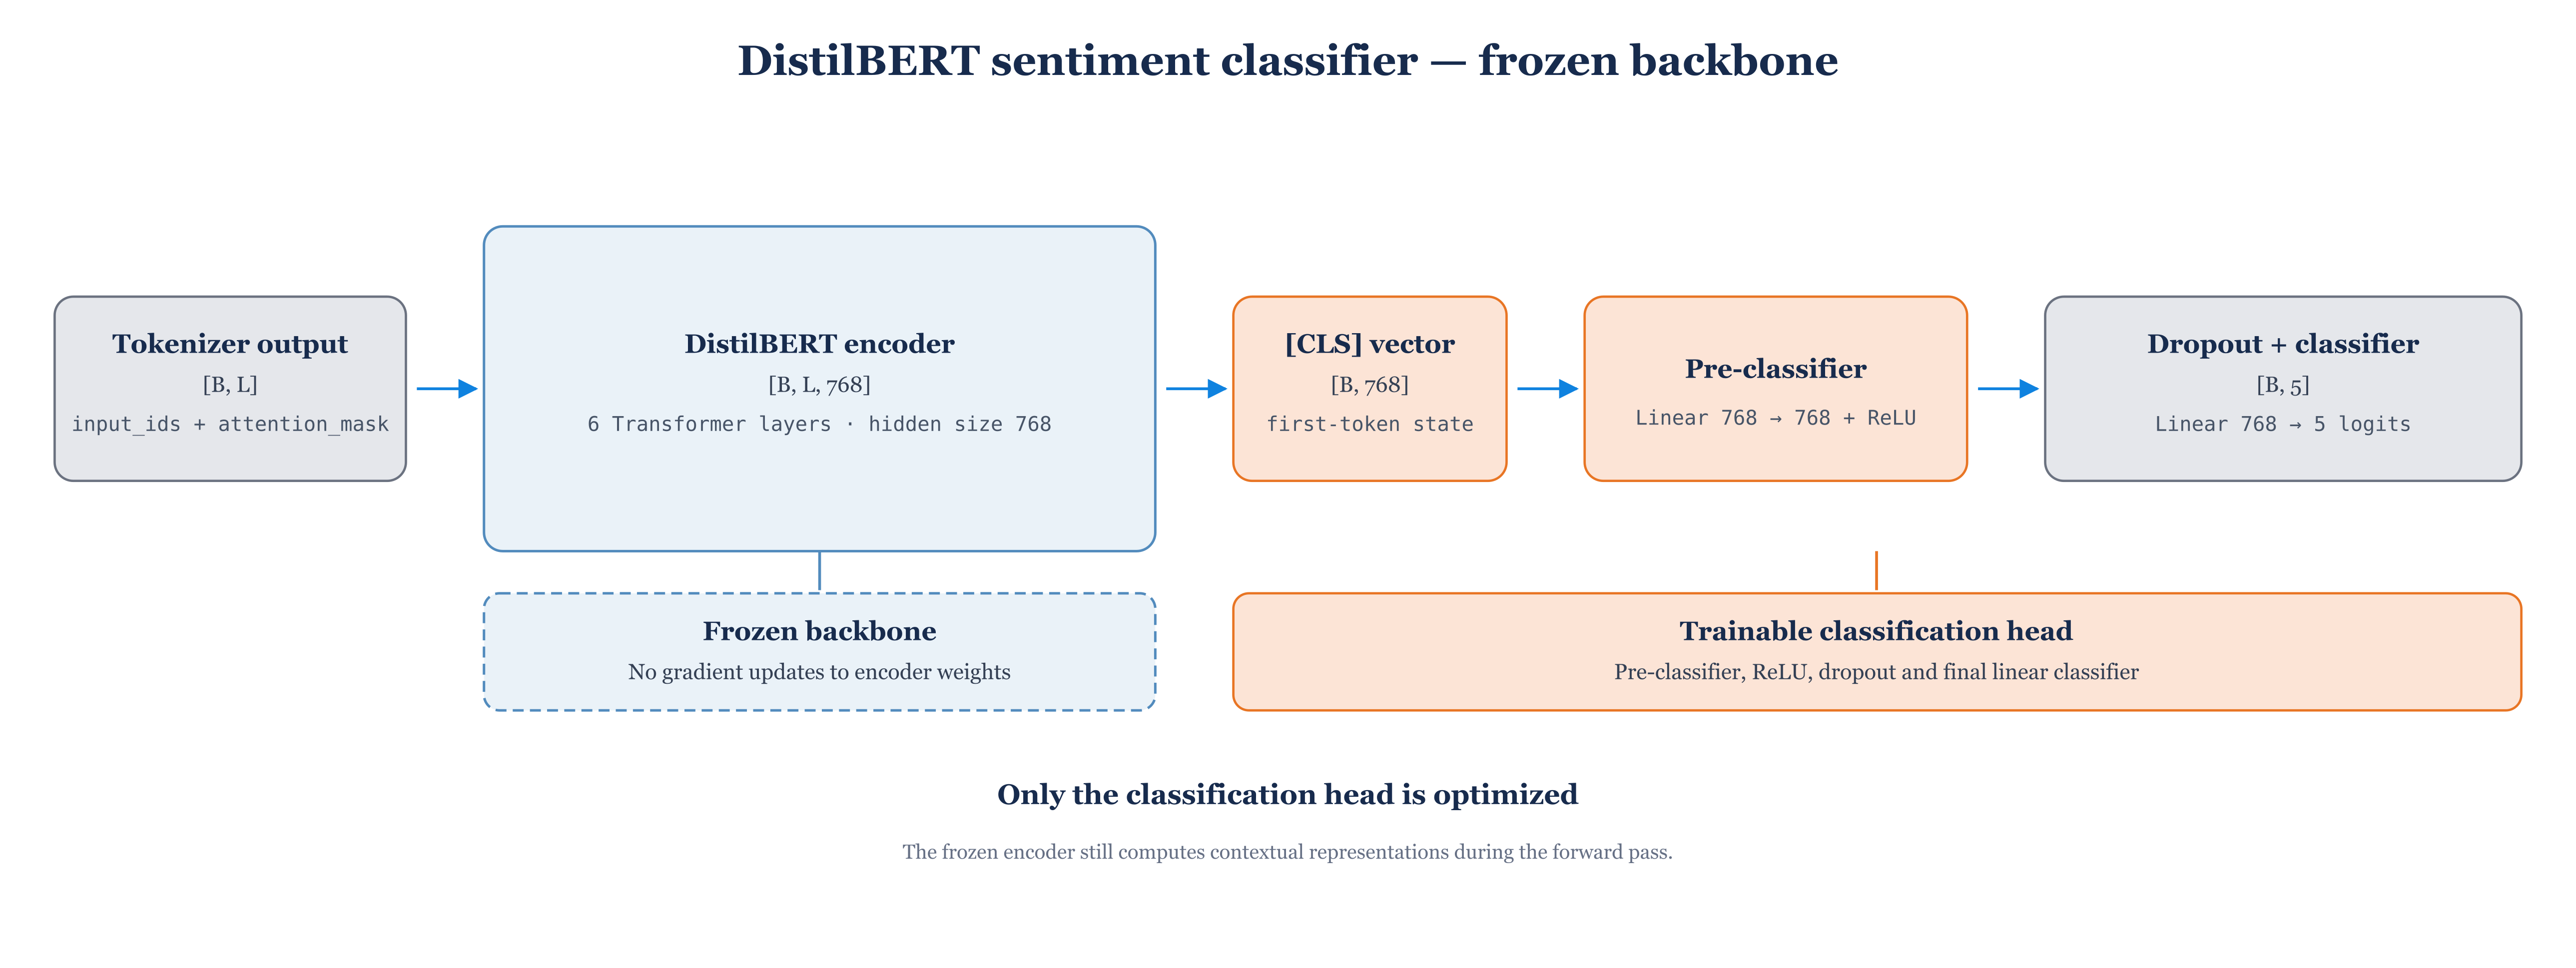
\includegraphics[width=\textwidth]{../../Assignment2/diagram-models/distilbert-frozen-model.png}
        \caption{DistilBERT with frozen backbone (EXP-2): only the classification head is trained.}
        \label{fig:distilbert_frozen_arch}
    \end{minipage}
    \hfill
    \begin{minipage}{0.48\textwidth}
        \centering
        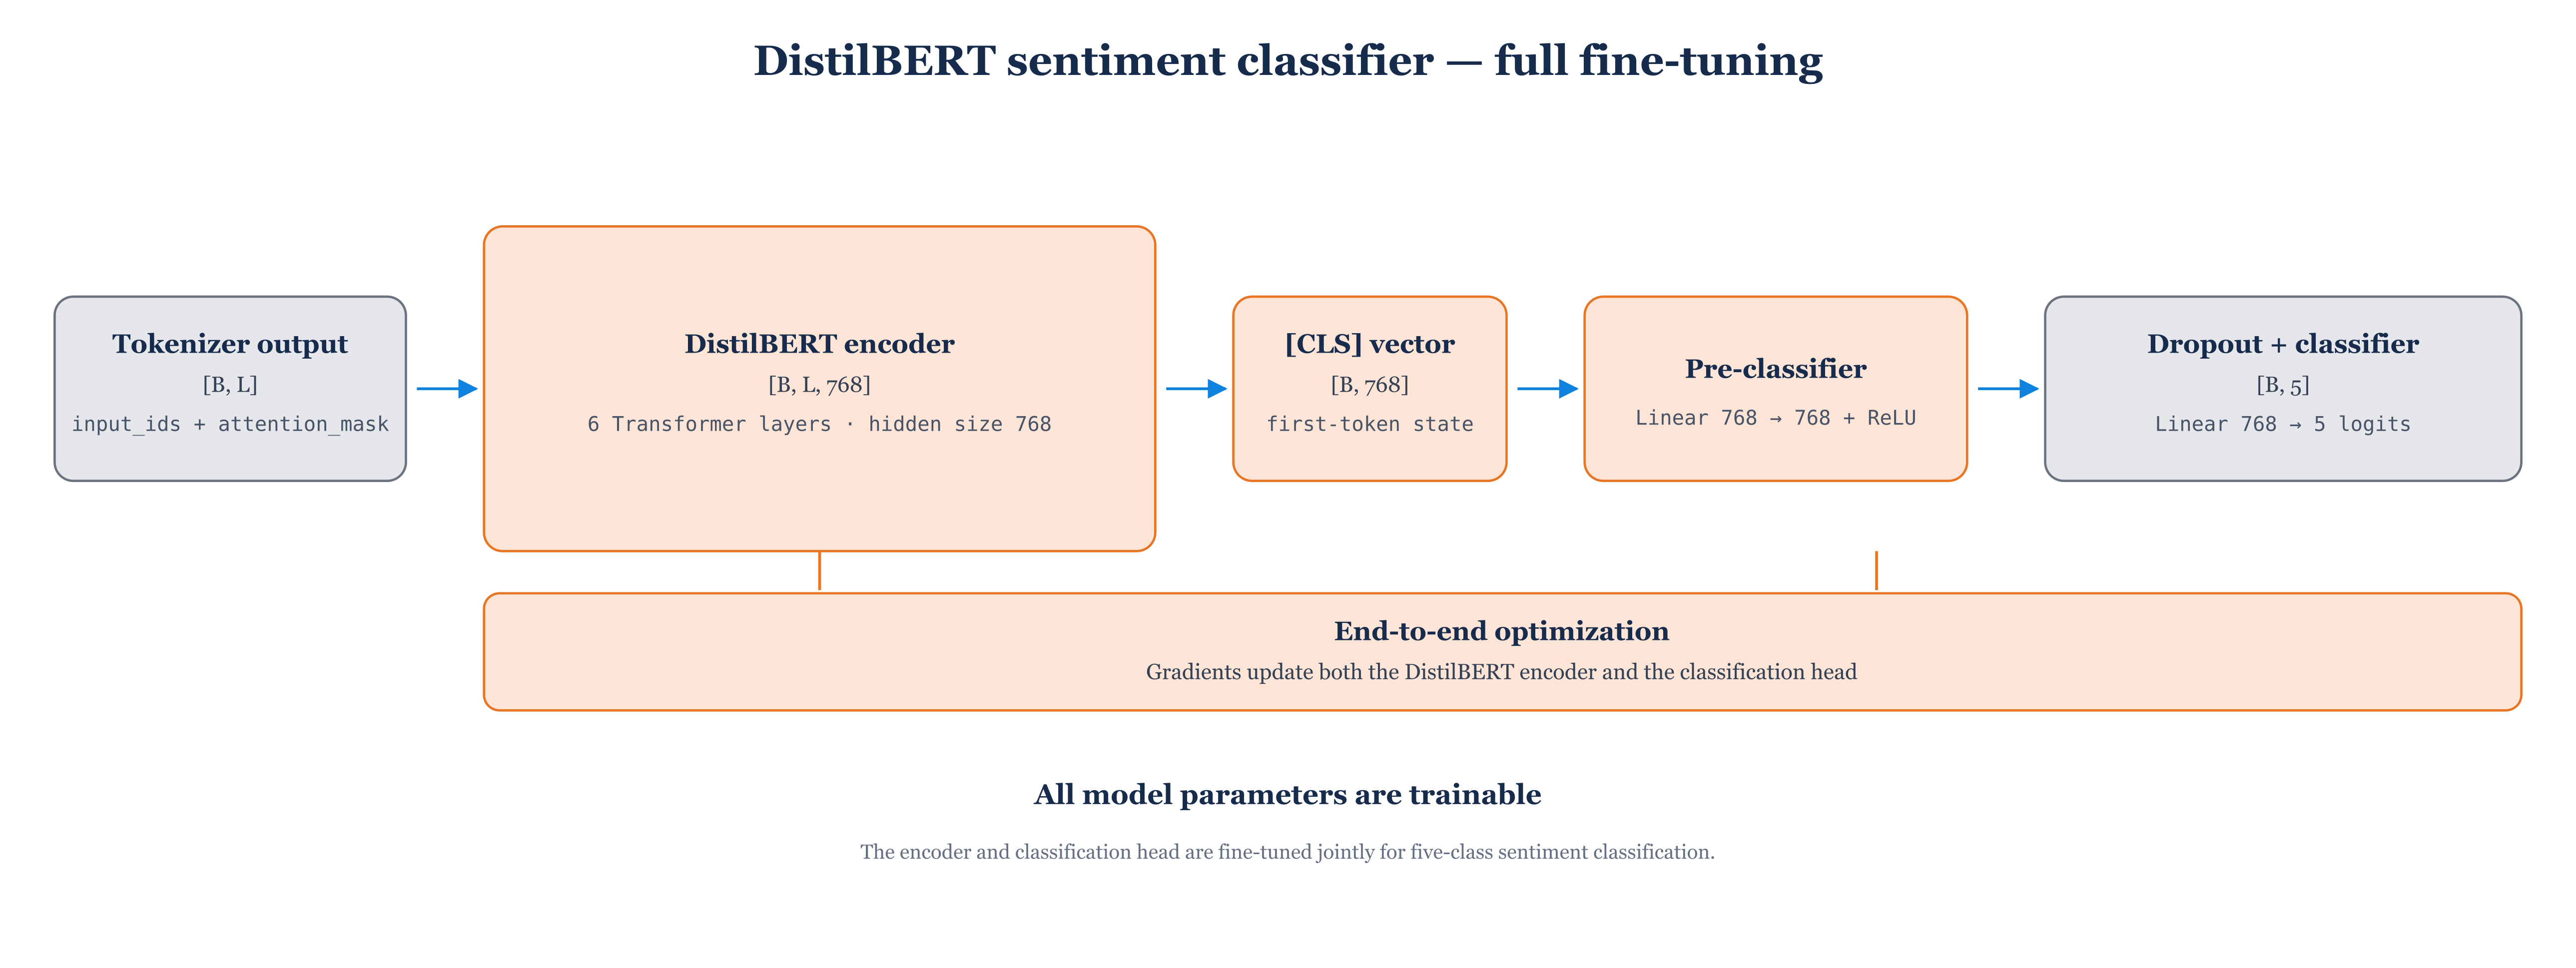
\includegraphics[width=\textwidth]{../../Assignment2/diagram-models/distilbert-full-model.png}
        \caption{DistilBERT with full fine-tuning (EXP-3): all parameters are updated.}
        \label{fig:distilbert_full_arch}
    \end{minipage}
\end{figure}
